\chapter{Resume Oracle APEX}
\section{Pembuatan Aplikasi Oracle Apex}
\begin{enumerate}

\item[1]Pergi ke Website Oracle APEX, https://apex.oracle.com, lalu klik Get Start For Free.

\begin{figure}[!htbp]
    \begin{center}
    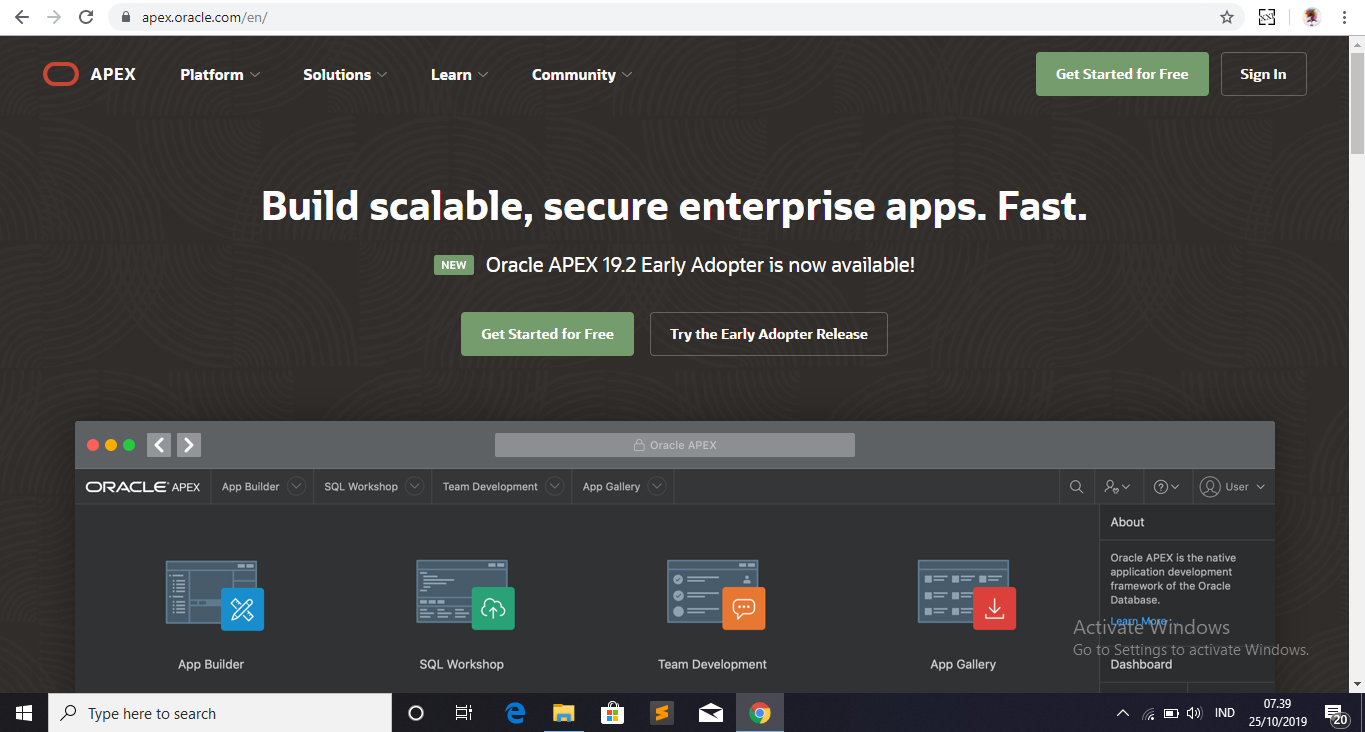
\includegraphics[scale=0.2]{apex/apex1.png}
    \caption{\textit{Get Started For Free.}}
    \end{center}   
    \end{figure}
    
\begin{figure}[!htbp]
\item[2]Pilih Request a Free Worksace.

    \begin{center}
    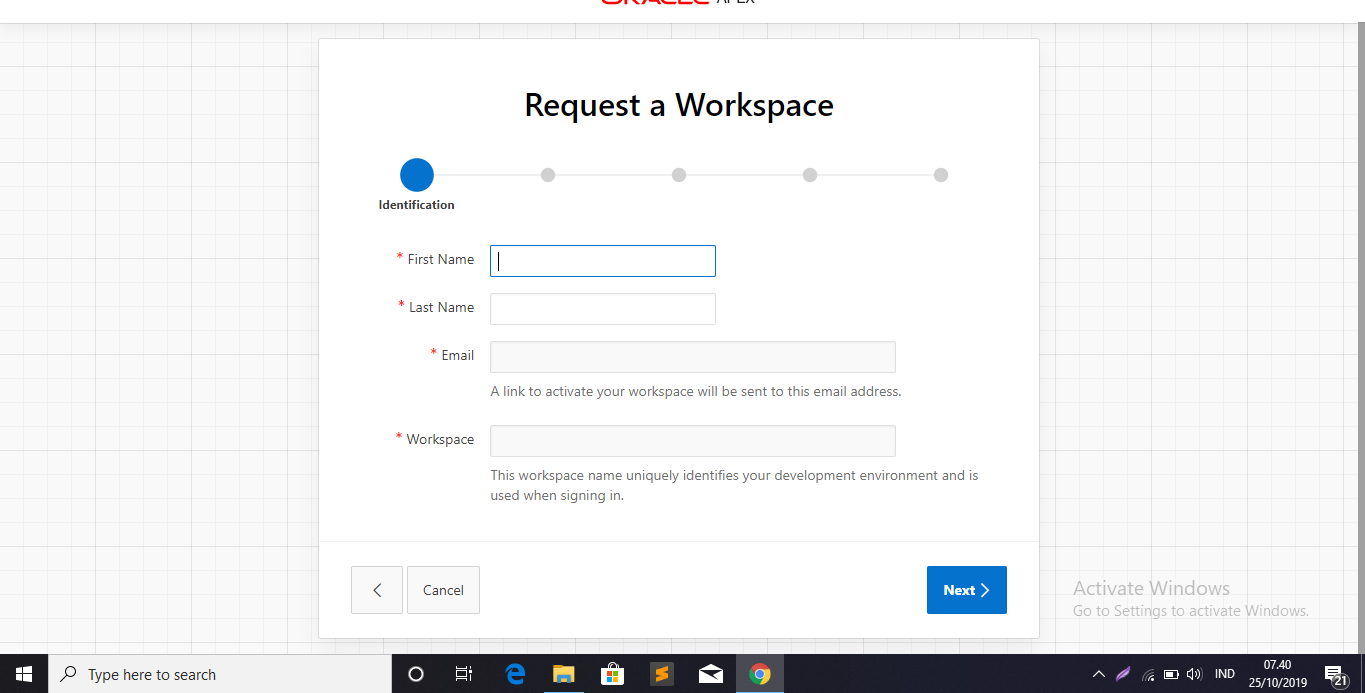
\includegraphics[scale=0.2]{apex/apex2.png}
    \caption{\textit{Request A Workspace.}}
    \end{center}
    \end{figure}
\begin{figure}
\item[3]Lengkapi data diri dan isi nama unik  untuk workspace.

        
\item[4]Centang, lalu pilih next.  

      
\item[5]Isi alasan pada kolom alasan merequest workspace, lalu next

 
\item[6] Centang Accept, lalu klik next.


\item[7] Tahapan terakhir untuk mengkonfirmasi apakah ini anda, lalu klik next.

   
\item[8] Workspace Sukses Dibuat.

    \begin{center}
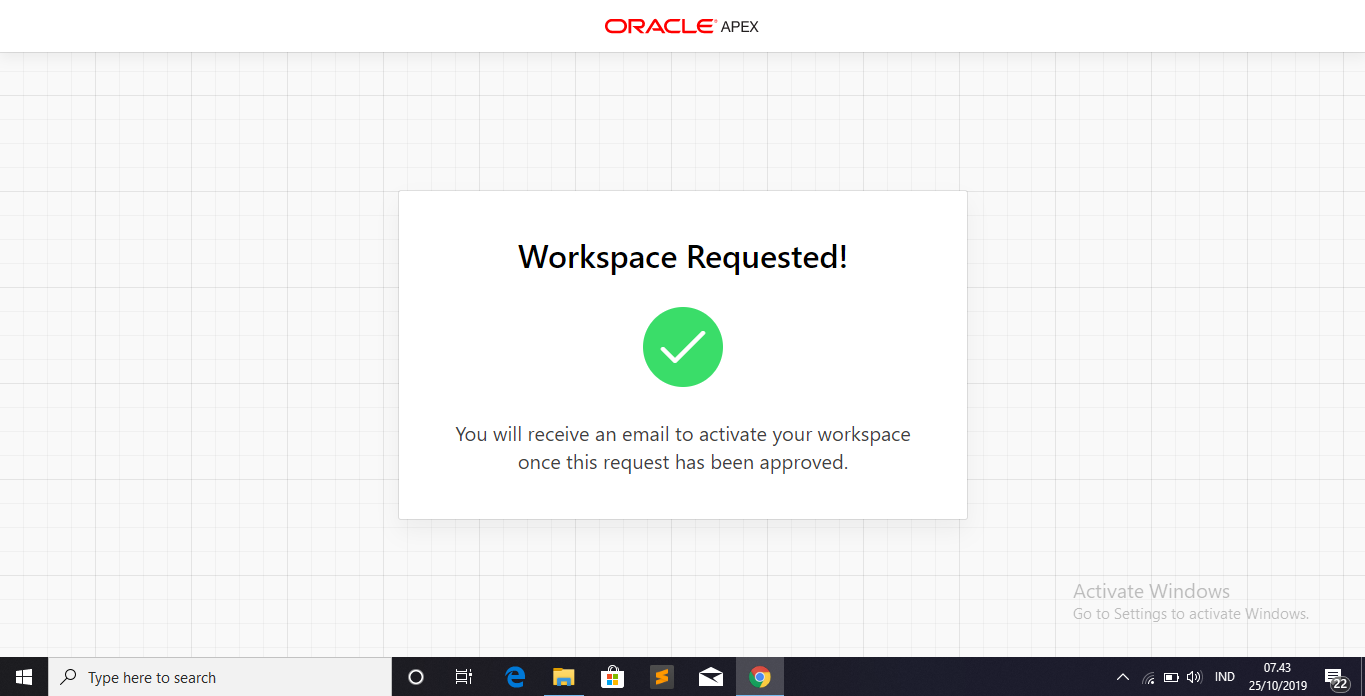
\includegraphics[scale=0.2]{apex/apex3.png}
    \caption{\textit{workspace sukses dibuat}}
        \end{center}
\label{gambar}
\end{figure}

\begin{figure}
\item[9] Email konfirmasi bahwa Workspace yang dibuat telah di Acc.

    \begin{center}
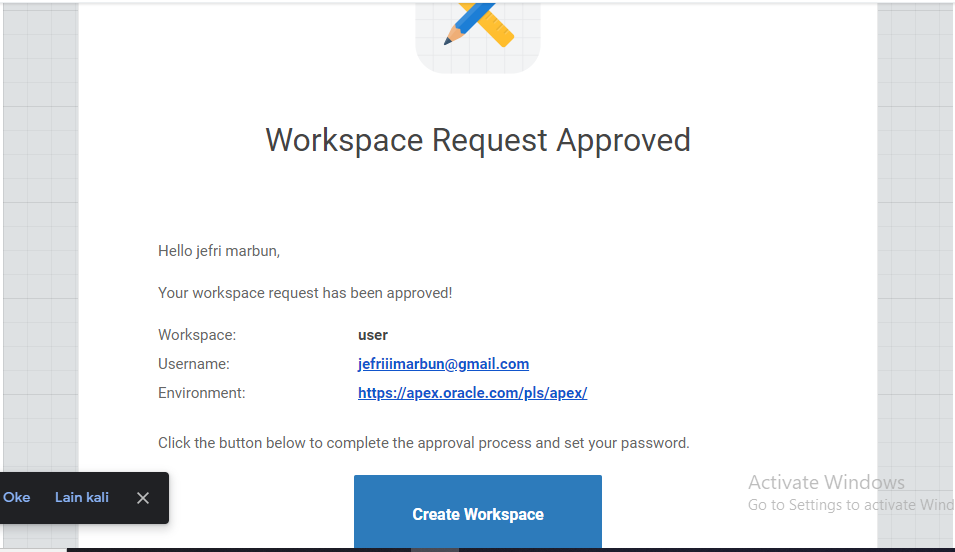
\includegraphics[scale=0.4]{apex/apex4.png}
    \caption{\textit{Email Acc.}}
        \end{center}
\label{gambar}
\end{figure}

\begin{figure}
\item[10] Workspace baru telah dibuat setelah itu lanjutkan dengan pilih create workspace dan isi dengan password baru.

    \begin{center}
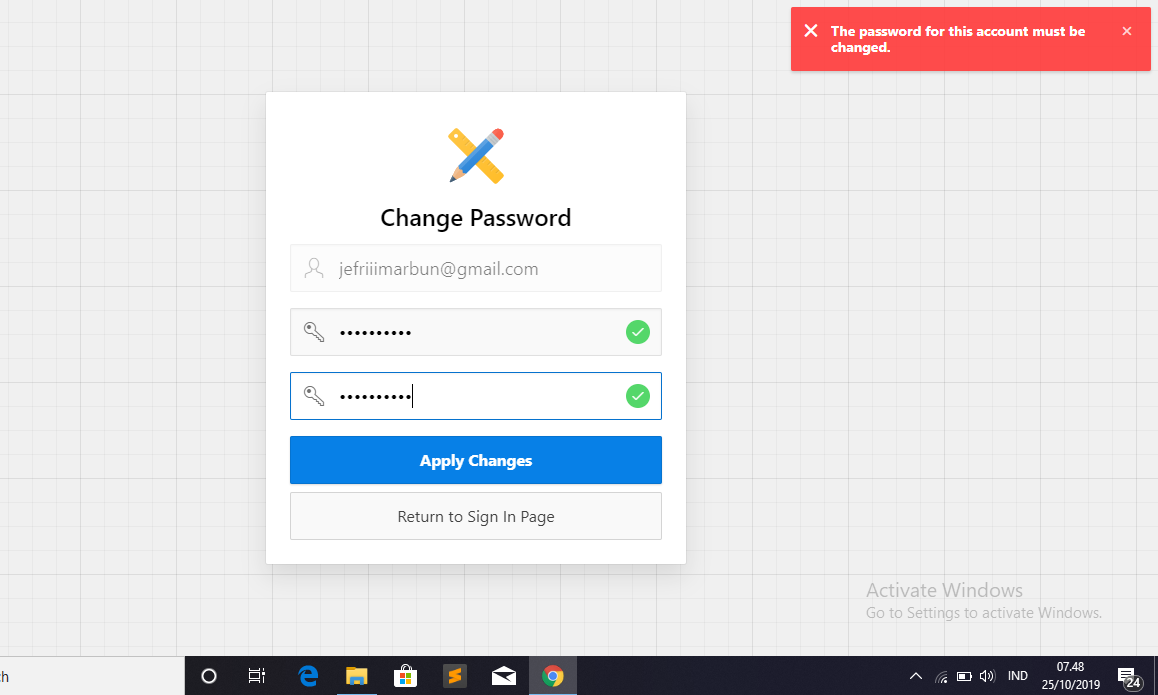
\includegraphics[scale=0.5]{apex/apex5.png}
    \caption{\textit{Pengisian password barul}}
        \end{center}
\label{gambar}
\end{figure}

\begin{figure}
\item[11] Lakukan Sign in akun workspace yang baru saja di buat.

\end{figure}

\begin{figure}
\item[12] Kita akan masuk ke tampilan awal


\end{figure}
\end{enumerate}

